In the previous chapter, we have decribed multiple unsupervised methods to analyze
multiview data.
As described in section~\ref{sec:srm:review}, the shared response
model~\cite{chen2015reduced} (SRM) is a multi-view latent factor model. It sees
the data $(\xb_i)_{i=1}^m$ as:
\begin{align}
  &\xb_i = A_i \sbb + \nb_i \\
  &A_i^{\top}A_i = I_p
    \label{eq:model:srm}
\end{align}
with $\nb_i \sim \Ncal(0, \Sigma_i)$ where $\Sigma_i = \sigma^2 I_v$ in
deterministic SRM and $\Sigma_i = \sigma_i^2 I_v$ in probabilistic SRM.

When working with high dimensional data, SRM is particularly
interesting as it provides a principled way to perform dimension reduction. Note that this
contrasts with ICA-like methods that do not incorporate dimension reduction in their model.

However SRM has initially been designed to work within regions of interest using
only few subjects. When using full brain data, computational costs become
high. In addition, memory requirements are difficult to meet since the full dataset needs to hold
in memory.

Fortunately, these high costs can be reduced. Intuitively, since the shared
response lives in a reduced space, a compressed representation of the input is
good enough to find a suitable estimate of the shared response.
FastSRM implements this idea. It turns out that there exists an optimal
compression of the input for which we can obtain the same solution as
with the full data.

\section{The FastSRM algorithm}
SRM algorithms use different set of parameters $\theta$ to represent the data.
In deterministic SRM $\theta = (A_i)_{i=1}^m, \sbb$ where $(A_i)_{i=1}^m$ are the
mixing matrices and $\sbb$ the shared response while in probabilistic SRM $\theta
= (A_i)_{i=1}^m, \Sigma_s, (\sigma_i)_{i=1}^m$ where $(A_i)_{i=1}^m$ are the
mixing matrices, $(\sigma_i)_{i=1}^m$ the noise levels and $\Sigma_s$ the
components variance.

In fMRI, the classical approach used to reduce the data is to apply an atlas.
Deterministic atlases~\cite{bellec2010multi} correspond to a parcellation of the
brain into $r$ regions. Reducing an image using a deterministic atlas corresponds to
averaging the signal within each region of the atlas. A probabilistic atlases such
as~\cite{dadi_fine-grain_2020} describes each region as a set of weights across
the full brain. Therefore, the image reduction can be done with a matrix product.

In FastSRM we consider a set of view specific atlases $U_i \in \RR^{v, r}$ such that
$U_i^{\top}U_i = I_r$ where $r$ is the number of regions in the atlas.
Data are reduced using $\zb_i = U_i^{\top} \xb_i$ and an SRM algorithm is applied
on data $\zb_i$ yielding parameters $\theta'$.
The figure~\ref{fig:srm:conceptual} illustrates this process.

Note that the parameters obtained with FastSRM $\theta'$ are different
from the parameters obtained with the corresponding SRM algorithm $\theta$ (the unmixing matrices in $\theta'$ do not even have the same shape as the unmixing matrices in $\theta$).
However, as we will see in the next section, there exists an explicit and exact
correspondence between $\theta$ and $\theta'$ although in the case of
probabilistic SRM, the algorithm applied on reduced data needs to be slightly modified in order to
obtain these guarantees. 

\begin{figure}
  \centering
  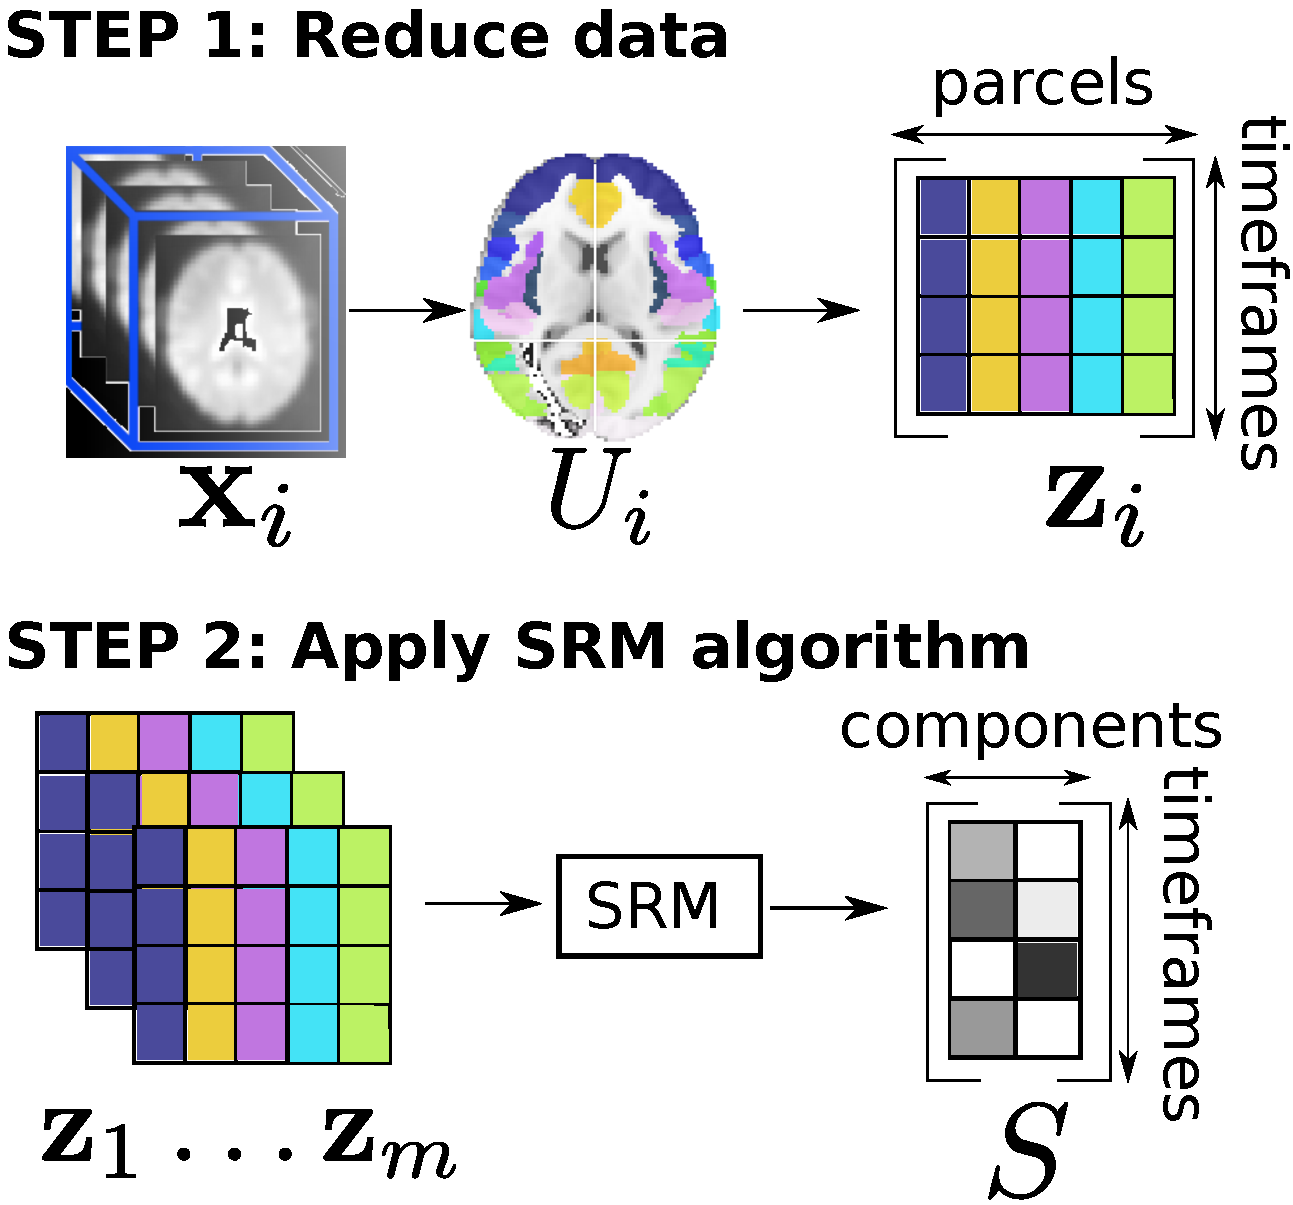
\includegraphics[scale=0.34]{figures/srm/conceptual_figure2.pdf}
  \caption{\textbf{FastSRM algorithm} In step 1, data $\xb_i$ are projected onto an
    atlas $U_i$ that may depend on the subject $i$ (top). In step 2 a SRM algorithm is applied on reduced data to compute the shared response.}
  \label{fig:srm:conceptual}
\end{figure}

From a computational stand point, the dimension reduction provides
a large reduction in memory usage. Indeed as the original data are seen only
once, it is no longer necessary to keep the full dataset in memory (we can load
data $\xb_i$ one after the other and similarly for the atlases $U_i$). Therefore
the memory consumption is only in $\bigO(vn)$ (where $v$ is the number of voxels
and $n$ is the number of samples) which is lower than SRM by a factor of $m$,
the number of subjects. The number of subjects is typically between $10$ and
$1000$. This yields a practical benefit: on fMRI datasets with many subjects, one no longer needs a large cluster to run the shared response model but only a modern laptop.
Additionally, low memory consumption reduces the
risk of thrashing~\cite{denning1968thrashing}, a phenomenon that causes large
increase in computation time when the memory used is close to the total available
memory in the hardware.

After preprocessing, the reduced representation $\zb_i$ is used instead of the
original data $\xb_i$ yielding a time complexity of $\bigO(
\mathrm{T_{preprocessing}} + \mathrm{n_{iter}} mpnr)$.
Let us highlight that in practice, it often happens that an experiment is run
multiple times such as when cross validated results are needed. In these cases,
the pre-processing is performed only once and the apparent complexity becomes
$\bigO(\mathrm{n_{iter}} mpnr)$ which is faster than SRM by
a factor of $\frac{v}{r}$. The number of regions in large atlases is about $r=1000$ and in full brain data, the number of voxels is about $300~000$ so that $\frac{v}{r}$ is typically about $1000$.

It remains to show how to draw a correspondence between FastSRM and SRM which is addressed in the following section.

\section{Optimal atlases}
In general, working with reduced data induces a loss of information and
therefore there is little hope to recover the parameters that would have been obtained from SRM from the parameters of FastSRM.
However, in this section, we show that there exists an optimal atlas in the sense that SRM and FastSRM yield the same results.

While it is possible in principle to use FastSRM with a sub-optimal atlas,
we will only use the optimal atlas and therefore, in the rest of the thesis, we refer to FastSRM with the optimal atlas as just FastSRM.

Let us consider $\xb_i = U_{\xb_i} \zb_i$ a PCA of $\xb_i$. As the number of
samples $n$ is lower than the number of features $U_{\xb_i} \in \RR^{v, n}$ and $\zb_i \in \RR^{n}$.  We also have $U_{\xb_i}^{\top}U_{\xb_i} = I$.
Therefore $U_{\xb_i}$ constitutes a possible choice of subject specific atlas.

As the next property shows, $U_{\xb_i}$ constitutes an optimal atlas when
fitting deterministic SRM.
\begin{prop}[Optimal dimension reduction via PCA for deterministic SRM]
  Let $(A_i)_i, \sbb$ be the solution obtained by deterministic SRM on data
  $\xb_i$ and $(A_i')_i, \sbb'$ the solution obtained by deterministic SRM on
  data $\zb_i = U_{\xb_i}^{\top} \xb_i$. Then $A_i = U_{\xb_i}A_i'$ and $\sbb = \sbb'$. 
\label{prop:optimaldetsrm}
\end{prop}
\begin{proof}
Updates of the mixing matrices $A_i$ in deterministic SRM
equation~\eqref{eq:detsrm:Aiupdate} can be written:
\begin{align}
  A_i &\leftarrow \Pcal(\xb_i \sbb^T)= U_{\xb_i}\Pcal(\zb_i \sbb^T)
  \label{eq:fastdetsrm:Aiupdate}
\end{align}
where $\Pcal$ is the projection on the Stiefel manifold: $\Pcal(M) = M
(M^{\top}M)^{-\frac12}$.


Therefore we can look for $A_i$ as $A_i = U_{\xb_i} \tilde{A_i}$. $\tilde{A_i}$ is
orthogonal. Indeed
\begin{align}
  &A_i^{\top} A_i = I_p \\
  & \implies \tilde{A_i}^{\top}U_{\xb_i}^{\top} U_{\xb_i} \tilde{A_i} = I_p \\
  & \implies \tilde{A_i}^{\top} \tilde{A_i} = I_p
\end{align}

Then, we use the fact that
\begin{align}
  \|\xb_i - A_i \sbb \|^2 = \| U_{\xb_i}\zb_i - U_{\xb_i}\tilde{A_i} \sbb\|^2 = \| \zb_i - \tilde{A_i} \sbb \|^2
  \label{eq:equality:xy}
\end{align}
Therefore, the solution of deterministic SRM on data $(\zb_i)_{i=1}^m$ and
$(\xb_i)_{i=1}^m$ are linked by the change of parameters $A_i = U_{\xb_i}A_i'$ and
$\sbb = \sbb'$ where $A_i' = \tilde{A_i}$. This concludes the proof.
\end{proof}

In the case of probabilistic SRM we can obtain very similar results. However the
algorithm applied on reduced data need to be slightly modified.
We call probSRM($\psi$) the probabilistic SRM algorithm modified such that
updates
\begin{align}
\sigma_i^2 \leftarrow \frac1{v} (\| \xb_i - A_i \EE[\sbb|\xb]\|^2 + \| \diag(\VV[\sbb | \xb]) \|^2)
\end{align}
are replaced by updates
\begin{align}
  \sigma_i^2 \leftarrow \frac1{\psi} (\| \xb_i - A_i \EE[\sbb|\xb]\|^2 + \| \diag(\VV[\sbb | \xb]) \|^2)
\end{align}

We have the following result:
\begin{prop}[Optimal dimension reduction via PCA for probabilistic SRM]
  Let $(A_i)_i, \sigma_i, \Sigma_s$ be the solution obtained by probabilistic SRM on data
  $\xb_i$ and $(A_i')_i, \sigma_i', \Sigma_s'$ the solution obtained by ProbSRM($v$) on
  data $\zb_i = U_{\xb_i}^{\top} \xb_i$.Then $A_i = U_{\xb_i}A_i'$, $\sigma_i =
  \sigma_i'$ and $\Sigma_s = \Sigma_s'$. 
  \label{prop:optimalprobsrm}
\end{prop}
\begin{proof}
  Updates of the mixing matrices $A_i$ in probabilistic SRM equation~\eqref{eq:psrm:Aiupdate}. We get:
  \begin{align}
    A_i &\leftarrow U_{\xb_i}\Pcal(\zb_i \EE[\sbb| \xb_i]^T)
    \label{eq:fastprobsrm:Aiupdate}
  \end{align}
  so we can look for $A_i$ as $A_i = U_{\xb_i} \tilde{A_i}$ and, as in the
  deterministic case, $\tilde{A_i}$ is orthogonal.
  Therefore equality~\eqref{eq:equality:xy} holds.
  
  Then we consider the negative log-likelihood of probabilistic srm:
  \begin{align}
    \loss &= \sum_i \frac12 v\log(\sigma_i^2) + \frac12 \log(|\Sigma_s|) + \int_{\sbb} \sum_i \frac1{2 \sigma_i^{2}}\|\xb_i - A_i \sbb \|^2 \\& \enspace + \frac12 \langle \sbb , \Sigma_s^{-1} \sbb \rangle  d\sbb \\
          &= \sum_i \frac12 v \log(\sigma_i^2) + \frac12 \log(|\Sigma_s|) + \int_{\sbb} \sum_i \frac1{2 \sigma_i^{2}}\|\zb_i - \tilde{A_i} \sbb \|^2 \\& \enspace+ \frac12 \langle \sbb , \Sigma_s^{-1} \sbb \rangle  d\sbb
  \end{align}
  where we use equality~\eqref{eq:equality:xy}.
  Optimizing the log-likelihood via expectation maximization yields the exact
  same updates as probabilistic srm on data $\zb_i$
  except that updates
  \begin{align}
    \sigma_i^2 \leftarrow \frac1{t} (\| \zb_i - \tilde{A_i} \EE[\sbb|\zb]\|^2 + \| \diag(\VV[\sbb | \zb]) \|^2)
  \end{align}
  are replaced by updates
  \begin{align}
    \sigma_i^2 \leftarrow \frac1{v} (\| \zb_i - \tilde{A_i} \EE[\sbb|\zb]\|^2 + \| \diag(\VV[\sbb | \zb]) \|^2)
  \end{align}

  The updates in both algorithms are linked  by $A_i = U_{\xb_i}A_i'$ where
  $A_i' = \tilde{A_i}$, $\sigma_i' =
  \sigma_i$ and $\Sigma_s'  = \Sigma_s$.

  This concludes the proof.
\end{proof}

The properties~\ref{prop:optimaldetsrm} and~\ref{prop:optimalprobsrm} show that
no information is lost by replacing $\xb_i \in \RR^v$ by its reduced representation $\zb_i \in \RR^n$.
A key property of the optimal atlas $U_{\xb_i}$ is that it is valid whether or
not the model for deterministic (respectively probabilistic) SRM holds.

A complexity analysis shows that finding the optimal atlas becomes the limiting
step of the pipeline. Even with fast implementations, the subject specific PCA
is costly. However FastSRM only works on $\zb_i$ so we do not need to know the value of $U_{\xb_i}$ straight away.
In practice, we observe data $X_i \in \RR^{v, n}$ and we want to get $Z_i
\in \RR^{n, n}$ such that $X_i = U_{\xb_i} Z_i$. This can be done by performing an
SVD of $X_i^{\top} X_i$ yielding $X_i^{\top}X_i= V_i D_i V_i^{\top}$ and setting $Z_i = D_i^{\frac12} V_i^{\top}$.
Although the product $X_i^{\top} X_i$ has complexity $\bigO(vt^2)$ there is
exactly $vt^2$ multiplications and additions so it costs a lot less than the PCA
on full data. When estimates of the mixing matrices are needed, they can be obtained by
applying equation~\eqref{eq:fastdetsrm:Aiupdate} in the deterministic SRM case and
equation~\eqref{eq:fastprobsrm:Aiupdate} in the probabilistic SRM case which only costs
$\bigO(mvp^2)$.
In practice the cost of the matrix products $X_i^{\top} X_i$ is often still the
limiting step of the pipeline (this depends on the number of iterations) but as
we show in the next chapter, this yields to great speed up compared to classical
SRM implementations. Note than if memory allows it, these matrix products can easily be done using multiple cores in parallel.

% In the next section, we investigate approaches to reduce the preprocessing time.

% \section{Efficient approximation of optimal atlases}
% As we have seen in the previous section, if $U_i = U_{\xb_i}$ where $\xb_i =
% U_{\xb_i} \zb_i$ is a PCA of $\xb_i$, then $U_i$ is an optimal atlas.
% A natural follow-up is to look for atlases that are close to optimal in the
% sense that the inertia $\| (I - U_i U_i^{\top}) \xb_i \|$ is low but are fast to
% compute and such that projecting data on the atlas is a cheap operation.

% Deterministic atlases are interesting as they allow for fast data projection
% (computing $U_i \xb_i$ only costs $\bigO(v)$). Furthermore, they are thought to
% be well-suited to fMRI data as they reduce noise via smoothing (this argument is
% detailed in~\cite{hoyos2018recursive}).
% %
% A first approach is to use existing deterministic atlases for fMRI data such as 
% ~\cite{schaefer2017local} or~\cite{bellec2010multi}. As theses atlases
% attempt to reduce the dimension of fMRI signals without losing too much signal,
% there is hope for the inertia to be small.
% RENA, the clustering approach
% of~\cite{hoyos2018recursive}, is also appealing as it is optimized to give low
% inertia while the cost of finding the deterministic atlas is low (computing $U_i$ only costs
% $\bigO(vn)$). As the number $r$ of regions increases, the inertia decreases
% and the approximation becomes better and better. An other possibility is to
% perform a PCA with a number of components $r < n$.

% The approaches previously described attempt to approximate $U_i$ by a
% deterministic atlas. Another possibility is to approximate directly $\zb_i$ via
% random projection.
% Let us call $X_i \in \RR^{v,
%   n}$ our data matrix. Following~\cite{mahoney2016lecture} (section 14.4), we
% can approximate $X_i^{\top} X_i$ by $\tilde{C} = \sum_{j \in \mathcal{J}} \frac1{p_j r} \xb_{ij}^{\top} \xb_{ij}$ where $\xb_{ij}$ is the $j$-th line of
%   $X_i$ and $\mathcal{J}$ is a set of $r$ indexes such that $\mathcal{J}$ contains
%   index $j$ with probability $p_j$. The most simple choice is $p_j=\frac1{v}$
%   which we use in our implementations. Other choices are possible, we refer the reader to section 15
%   of~\cite{mahoney2016lecture} for more details.  Computing an approximation of $X_i^{\top} X_i$ is interesting
%   because the SVD of $X_i^{\top} X_i$ allows us to recover the reduced data
%   $Z_i$ up to an irrelevant sign indeterminacy. 
%   If spatial maps $A_i$ are needed, they can be recovered from the data using the formula
%   $A_i \leftarrow \mathcal{P}(\xb_i \sbb^{\top})$ (in the deterministic SRM case) or
%   $A_i \leftarrow \mathcal{P}(\xb_i \EE[\sbb^{\top}|\xb])$ (in the probabilistic SRM case).

  Up to now, we have assumed that the covariance of components is diagonal in
  probabilistic SRM. In the next section we justify this assumption.

\section{Identifiablity of the shared response model}
We first show why deterministic SRM and probabilistic SRM without any
restriction on the covariance of the components can
only recover unmixing matrices up to an arbitrary rotation.

Let us consider data $\xb_i$ generated from deterministic SRM with
mixing matrices $A_i$, shared response $\sbb$ and noise covariance $\sigma$.
Then, deterministic SRM with parameters $A'_i = A_i \theta$ and $\sbb' = \theta^{\top} \sbb$ where
$\theta \in \RR^{k, k}$ is an orthogonal matrix also
generate $\xb_i$.

Similarly, in the probabilistic SRM case, if data $\xb_i$ are generated from the
probabilistic SRM model with 
parameters $A_i$, $\Sigma_s$, $\sigma_i^2$ (where $\Sigma_s$ can be any
symmetric positive definite
matrix) then the probabilistic SRM model with parameters $A_i\theta$, $\theta^{\top} \Sigma_s \theta$, $\sigma_i^2$  where
$\theta \in \RR^{k, k}$ is an orthogonal matrix also generate $\xb_i$.

Then, we show that if the covariance of the components are diagonal, under some
assumptions probabilistic SRM is identifiable:
\begin{prop}[Identifiability of probabilistic SRM]
  \label{prop:fastsrm:identifiability}
  Let $\xb_i$ be generated from the probabilistic SRM model with parameters 
  $A_i$, $\Sigma_s$, $\sigma_i^2$ (where $\Sigma_s$ is diagonal positive with
  distinct values on the diagonal) and assume there exists another set of parameters $A_i'$, $\Sigma_s'$,
  ${\sigma_i'}^2$ (where $\Sigma_s'$ is diagonal positive with
  distinct values on the diagonal) that also generate $\xb_i$.
Then if $m\geq 3$, $A_i' = A_i P^{\top}$, $\Sigma_s'= P\Sigma_sP^{\top}$ and
  ${\sigma_i^2}' = {\sigma_i}^2$ where $P$ is a sign and permutation matrix
  independent (the same for all subjects).
\end{prop}
\begin{proof}
  Let us consider $\EE[\xb_i \xb_j^{\top}]$ for $i \neq j$.
  We have:
  \begin{equation}
  A_i \Sigma_s A_j^{\top} = A_i' \Sigma_s' {A_j'}^{\top}
  \label{eq:fastsrm:svd}
  \end{equation}
  up to re-ordering, equation~\eqref{eq:fastsrm:svd} gives two singular value
  decompositions of the same matrix.
  Therefore, by unicity of the singular value decomposition we have:
  $\Sigma'_s = P_i \Sigma_s P_j^{\top}$ and $A_i' = A_i P_i^{\top}$ and $A_j =
  A_j P_j^{\top}$ where $P_i$ and $P_j$ are sign and permutation matrices.
  Since there are more than three subjects, there exists subject $z$ such that
  $\Sigma'_s = P_i \Sigma_s P_z^{\top}$ and therefore
  $P_i \Sigma_s P_z^{\top} =  P_i \Sigma_s P_j^{\top}$ so that $P_j =
  P_z$. So all sign and permutations are the same and we call $P$ their
  common value.
  Then we consider
  $\EE[\xb_i \xb_j^{\top}] = A_i \Sigma A_i^{\top} + \sigma^2 I_v = A_i' \Sigma_s'
  {A_i'}^{\top} + {\sigma^2}' I_v$
  so we get ${\sigma^2}' = {\sigma^2}$
\end{proof}

Proposition~\eqref{prop:fastsrm:identifiability} justifies that
$\Sigma_s$ should be assumed to be diagonal in probabilistic SRM.
In addition, working with a diagonal covariance matrix allows to speed up
slightly the computations (although this does not change the time complexity of
the algorithm).

In the next chapter, we investigate how FastSRM works in practice compared to
available implementations.
